\section{Task identity and physical acceptance}
\label{chapter:03}

% block-id: auto.03.p1
\hypertarget{auto.03.p1}{}
A task submission specifies a case, parameter file, run identifier, and resource policy. A long task first returns its identifier and then persists status, logs, and results in its assigned directory. After a client timeout, the client queries that run rather than interpreting a communication failure as solver termination and starting another solve. Results retain both execution status and physical acceptance; cancellation, budget exhaustion, program exceptions, and lack of convergence retain their respective causes.

% block-id: auto.03.p2
\hypertarget{auto.03.p2}{}
The runner manages the process tree it creates and binds cancellation and cleanup to process creation identity. The project budget is eight logical processors, 24 GiB of task memory, and an 8 GiB system free-memory reserve. Student cases additionally obey their actual license constraints and request four solver cores. Resource records explain execution capacity and termination causes so that constrained runs can be interpreted separately from completed calculations. \cite{PSUTIL,PYTHON}

% block-id: auto.03.p3
\hypertarget{auto.03.p3}{}
Recovery first checks the identities of the request, source snapshot, and checkpoint. Existing tutorial recovery reruns saved inputs under a linked new identifier; complete numerical routes use their own checkpoint protocols. Reconnecting a client, restarting a task, and restoring a numerical checkpoint have different meanings, which are retained in parent-task relationships and recovery descriptions.

% block-id: auto.03.p4
\hypertarget{auto.03.p4}{}
Physical conventions enter each execution interface through the common parameter file: SI units, exp(jωt), RMS phasors, copper at 20 °C, σ=5.8×10⁷ S/m, and μr=1. The principal transport condition is 200 kHz and 20 A RMS. Strands are insulated along their lengths and connected in parallel at their ends. Common terminal voltage and total current jointly determine complex strand currents through the augmented system below.

% block-id: auto.03.equation
\hypertarget{auto.03.equation}{}
\hypertarget{E04}{}\begin{equation}\begin{bmatrix} Z&-\mathbf1\\ \mathbf1^T&0\end{bmatrix}\begin{bmatrix}\mathbf i\\V\end{bmatrix}=\begin{bmatrix}-\mathbf e\\I_t\end{bmatrix}\tag{1}\label{eq:E04}\end{equation}

% block-id: auto.03.p5
\hypertarget{auto.03.p5}{}
Here Z is the selected model's coupled impedance matrix, e contains independently induced voltages, and i and V are the unknown complex currents and terminal voltage. Acceptance checks current constraints, power balance, and discretization sensitivity, together with return and boundary conditions. The 2 mm round wire in Q1 serves as an analytical calibration and has a DC current density of approximately 6.366 A/mm²; Q2 candidates require at least 5 mm² nominal copper area. Small-strand port cases validate interfaces and constraints, with their area conditions retained in the case description.

% block-id: auto.03.figure
\hypertarget{auto.03.figure}{}
\begin{figure}[!htbp]
\centering
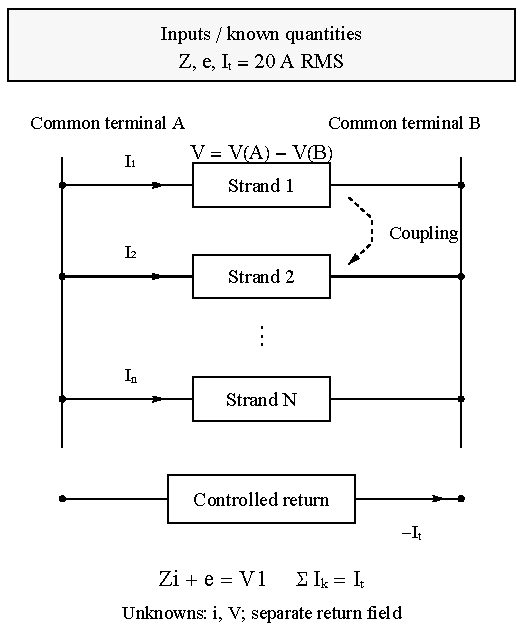
\includegraphics[width=\linewidth,height=.72\textheight,keepaspectratio]{../../assets/en/common_terminal.pdf}
\caption{Multistrand common terminals and return. Strands are insulated along their paths and connected in parallel at both ends; their phasor currents follow from the common voltage and total-current constraints. The coupling matrix Z and excitation term e contain the impedance and field contributions retained by the model. The controlled return carries the opposite total current and has its own terminal field. Known inputs and unknown currents and voltage are identified.}
\label{fig:common_terminal}
\end{figure}
